\documentclass[11pt]{article}
\usepackage[margin=1in]{geometry}
\usepackage{amsmath,amssymb,booktabs,graphicx,hyperref,array,microtype,enumitem}
\newcommand{\Orbits}{6720}
\newcommand{\OrbitsF}{5040}
\newcommand{\OrbitsM}{1680}
\newcommand{\FCyc}{152}
\newcommand{\FEsc}{1410}
\newcommand{\FHor}{26}
\newcommand{\FStuck}{3452}
\newcommand{\MEsc}{476}
\newcommand{\MHor}{34}
\newcommand{\MStuck}{1170}
\newcommand{\Succ}{1373}
\newcommand{\SuccF}{1027}
\newcommand{\SuccM}{346}
\newcommand{\SuccPrefixes}{56}
\newcommand{\FibHits}{0}
\newcommand{\AnyConsHits}{0}
\newcommand{\NonCyc}{1946}
\newcommand{\XLaw}{448}
\newcommand{\DomN}{5435}
\newcommand{\ExtN}{150}
\newcommand{\NLabels}{46}
\newcommand{\NbCheck}{3000}
\newcommand{\LocN}{14774}
\newcommand{\IntBytes}{4103}
\newcommand{\RuleBytes}{75}
\newcommand{\RuleZ}{64}
\newcommand{\CandStep}{84.1}
\newcommand{\GramBits}{8.49}
\newcommand{\FibTab}{16906}
\newcommand{\FibTabZ}{3118}
\newcommand{\FibCode}{5219}
\newcommand{\FibMoves}{8.25}
\newcommand{\FibOps}{26937}
\newcommand{\FibRec}{5.08}
\newcommand{\FibStates}{201}
\newcommand{\SqDTab}{12093}
\newcommand{\SqDTabZ}{946}
\newcommand{\SqDCode}{5457}
\newcommand{\SqDMoves}{4.37}
\newcommand{\SqDOps}{46}
\newcommand{\SqDRec}{0.75}
\newcommand{\SqDStates}{85}
\newcommand{\SqWTab}{7375}
\newcommand{\SqWTabZ}{870}
\newcommand{\SqWCode}{9765}
\newcommand{\SqWMoves}{6.92}
\newcommand{\SqWOps}{31}
\newcommand{\SqWRec}{0.38}
\newcommand{\SqWStates}{45}

\title{\textbf{UNNS-U2-TI}\\[2pt]\large Target-Blind Selector Language and Generative Knowledge Accounting}
\author{UNNS Research Collective}
\date{Version v001 \quad (addendum to UNNS-U2-KI v001, which is frozen; R3, FP-SYM and earlier releases are unchanged)}
\begin{document}\maketitle
\begin{abstract}\noindent
KI v001 measured how much mathematical knowledge three route selectors use. This addendum asks the converse: what do fixed, sequence-independent, graph-local rules produce on their own? \textbf{TI-0.} The exact-arithmetic gate passes: all \NLabels{} route-label expressions have integer coefficients and no executed selector uses floating point. This corrects a precaution stated in KI v001. \textbf{TI-1.} We freeze a grammar GL-1 with 360 finite-control rules (class F, \OrbitsF{} orbits over 14 starts) plus a reference class M with unbounded memory (120 rules), and audit that no rule reads a target, step counter or table. \textbf{TI-2.} In the registered run of \Orbits{} orbits, \Succ{} orbits meet the registered success criterion, but they come from only \SuccPrefixes{} distinct prefixes and are geometric growth ($\times4$ or $\times25$ per two steps). No orbit reproduces Fibonacci numbers, consecutive squares, primes, triangular numbers or consecutive members of any registered family. \textbf{TI-3.} Under a fixed encoding, a graph-local rule costs \RuleBytes{} bytes plus a \IntBytes-byte interpreter and no sequence-specific table; the knowledge-rich selectors use $\geq$\SqWTabZ{} compressed table bytes. These numbers describe different tasks and are not a complexity comparison. Target-independent generation of a nontrivial sequence is \emph{not} shown.
\end{abstract}

\section{Scope and evidence levels}
\emph{Certified exactly}: TI-0 (integer polynomial coefficients, exact comparison against the frozen evaluator). \emph{Tested}: the registered run, the audits, the accounting. \emph{Exploratory}: analyses added after results were seen (labelled where they occur). ``No hit in the registered vocabulary'' is never read as impossibility.

\section{TI-0: exact-arithmetic gate}
All \NLabels{} label expressions of the three KI selectors were evaluated as integer Horner forms from the stored coefficient polynomials. There are zero non-integer coefficients and zero labels with division or float literals. A static AST scan of the executed selector sources finds only true-division nodes in SymPy symbolic code and Fraction arithmetic. On \DomN{} inputs (squares $n^2$, $n$ up to $10^{15}$) the exact evaluator, the KI shortcut evaluator and the frozen lambdified evaluator agree on every move sequence and final state; on \ExtN{} random $n\in[10^{10},10^{60})$ they also agree. A float trap confirms the exact path raises on any float.

\paragraph{Correction.} KI v001 listed floating-point evaluation of the U2-001 labels as a caveat. TI-0 shows the labels are exact integers, so the caveat was a precaution that did not materialize. KI v001 stays frozen; this paragraph is the correction.

\section{TI-1: the language GL-1 and target-blindness}
A rule is a tuple (dir, hist, band, key, order). At vertex $x$ it enumerates graph neighbours $y$ (from divisors and square divisors of $x$), filters by direction, by the band ($y\le2x$, $y\ge x/2$, or both) and by the last $\le2$ vertices (class F) or the whole visited set (class M), then picks the min or max of a key ($y$, $N$, $y\bmod4$, $y\bmod6$, $v_2(y)$), ties by smallest $y$. Information channels are X (current vertex), H (window $\le2$), NB (neighbours), and for M only V (visited set). Horizon $T=400$ and escape bound $10^{18}$ act outside the selector.

\paragraph{Target-blindness conditions.} TB1 no target or table is an input; TB2 no step counter; TB3 the same rule is applied to every start; TB4 class F reads only X, H, NB; TB5 the interpreter holds no sequence constants. \emph{Audit} (verified by script): neighbour sets agree with an independent trial-division engine for $x\le3000$ (0 mismatches); \LocN{} class-F states re-executed from $(x,\text{hist})$ alone reproduce the step (0 mismatches); appending history beyond the window never changes a step (0 mismatches); class F made 0 reads of V; the interpreter imports only \texttt{sys} and the graph library, reads no file, and has integer literals $\{0,1,2,4,6\}$ only. This audits the declared language, not every conceivable hidden dependency.

\paragraph{Registration.} Config, interpreter and recognizers are SHA-256 pinned; the verifier checks the hashes and that the stored results equal a fresh re-run. Recognizers: Berlekamp--Massey over $\mathbb Q$ (order $\le4$) on the first 60 terms, and family tests on naturals, squares, cubes, triangular numbers, $2^k$, $3^k$, Fibonacci, factorials and primes. \textbf{Amendment A1} reduced the BM window from 400 to 60 terms after a timing test of a single rule hung on large integers; this was made before any complete run, and the only endpoints seen were from that one rule.

\section{TI-2: what the rules produce}
\begin{center}\small\begin{tabular}{lrrrr}\toprule
class & cyclic & escape & horizon & stuck\\\midrule
F (360 rules) & \FCyc & \FEsc & \FHor & \FStuck\\
M (120 rules) & 0 & \MEsc & \MHor & \MStuck\\\bottomrule\end{tabular}\end{center}
(14 starts per rule, \Orbits{} orbits.) \Succ{} orbits (F \SuccF, M \SuccM) satisfy the registered success criterion (a linear recurrence of order $\le4$, or consecutive family members, with no cyclic ending). Their sequences are:
\begin{itemize}[itemsep=1pt]
\item $1,4,16,64,256,\dots$ (move $+1$ repeated; recurrence $a_n=4a_{n-1}$);
\item $3,12,75,300,1875,7500,\dots$ (alternating $+1$, $+4$; $\times25$ every two steps);
\item the same pattern with periodic exceptions (e.g.\ $4,18,147,588,\dots$).
\end{itemize}
All successes are of these forms. \textbf{This is trivial geometric growth, not evidence that the rules generate the intended sequences.} No orbit reaches Fibonacci (\FibHits{} consecutive-Fibonacci hits), and \AnyConsHits{} orbits show consecutive members of any registered family. Family ``subset'' hits (naturals, powers of 2, squares) are weak signals: a ``subset'' needs only 8 family members among the terms, and no consecutive run was found.

\paragraph{Exploratory (after the registered results).} Of \NonCyc{} non-cyclic orbits that escape or hit the horizon, \XLaw{} follow $x\mapsto(x+1)^2$ (e.g.\ $1,4,25,676,458329,\dots$). These are \emph{not} registered successes because they leave the $10^{18}$ bound after about 7 terms, so the registered recognizers never see enough terms. The map $x\mapsto(x+1)^2$ is a one-line law; it is not a target sequence.

\section{TI-3: knowledge accounting (fixed encoding)}
Encoding: canonical minified JSON of the data each selector consults; zlib level 9 as a rough proxy; code bytes = UTF-8 selector source size.
\begin{center}\small\begin{tabular}{lrrrrrr}\toprule
selector & table B & zlib B & code B & states & moves/step & ops/step\\\midrule
Fibonacci successor (KI) & \FibTab & \FibTabZ & \FibCode & \FibStates & \FibMoves & \FibOps\\
Squares direct (KI) & \SqDTab & \SqDTabZ & \SqDCode & \SqDStates & \SqDMoves & \SqDOps\\
Squares wrapper (KI) & \SqWTab & \SqWTabZ & \SqWCode & \SqWStates & \SqWMoves & \SqWOps\\
Graph-local rule (class F) & \RuleBytes & \RuleZ & \IntBytes & --- & 1 & \CandStep{} cand.\\\bottomrule\end{tabular}\end{center}
A class-F rule is $\log_2 360\approx\GramBits$ bits of choice. \emph{Caution:} the knowledge-rich selectors route to a prescribed target (the next Fibonacci number or square); the graph-local rules do not, and they never produce those targets. A smaller table is therefore not evidence of lower intrinsic complexity: the graph-local rules simply solve a different, easier problem. The honest reading is that the information the TI rules lack is exactly what the KI selectors store.
\begin{center}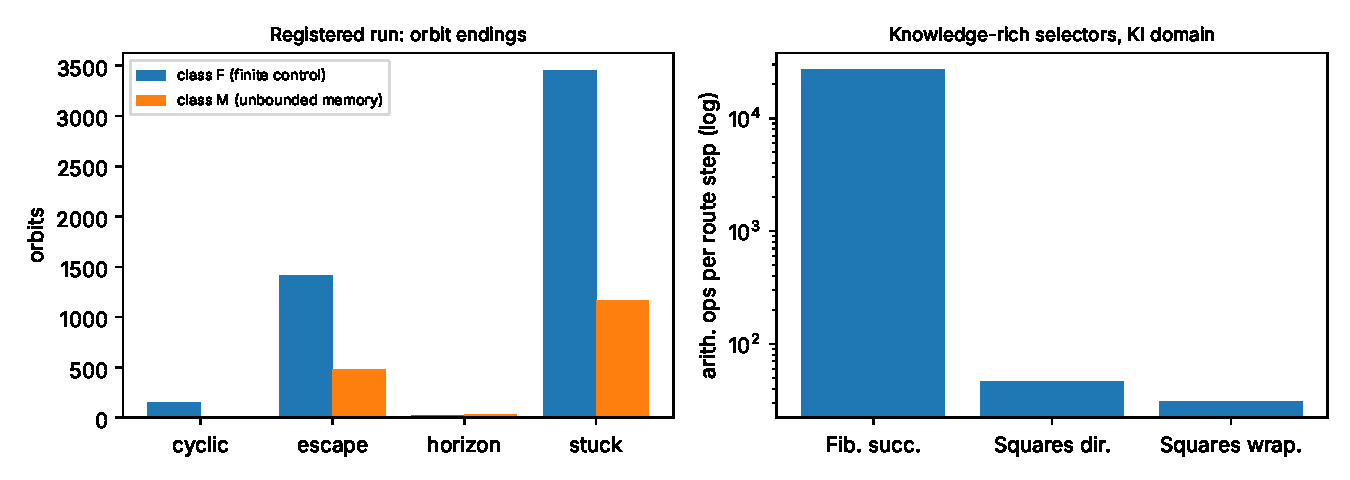
\includegraphics[width=.9\textwidth]{../figures/ti_summary.pdf}\end{center}

\section{The R3$'$ decision}
R3$'$ (exact integer $+,-,\times$, division by constants, comparison, $\mathrm{isqrt}$, residues) is adopted as a separate, named \emph{algebraic-monotone selector class}. Definition 2.1 of R3 is not modified retroactively.

\section{Gates, assumptions, consequences}
Gates passed: TI-0 exact (0 mismatches), registration hashes, stored equals fresh (\Orbits{} orbits), neighbour/locality/perturbation audits. Unverified: that GL-1 exhausts target-blind finite-control rules (it does not); that other recognizers would find nothing; behaviour beyond $T=400$ or $10^{18}$; whether richer grammars or interpreters generate primes. Consequences: within GL-1 no nontrivial target sequence is generated; ``target-independent intrinsic generation'' remains open. The unresolved quadratic-tower cases and class-11 optimization are separate follow-ups, not prerequisites.
\end{document}
